\documentclass[11pt]{article} % use larger type; default would be 10pt
\usepackage[utf8]{inputenc} % set input encoding (not needed with XeLaTeX)
\usepackage{amsmath}
\usepackage{fullpage}
\usepackage{mathtools}
\usepackage{enumitem}
\newcommand{\drv}[2]{\ensuremath{\frac{\partial #1}{\partial #2}}}
\newcommand{\ddrv}[2]{\ensuremath{\frac{\partial^2 #1}{\partial #2^2}}}

\usepackage{graphicx}
\usepackage{caption}
\usepackage{subcaption}

\title{UQ on Two-Group, 2D Criticality Diffusion\\ \normalsize A simple problem for testing and learning}
\author{Paul Talbot}
%\date{} % Activate to display a given date or no date (if empty),
         % otherwise the current date is printed 

\begin{document}
\maketitle
\section{Introduction}
While the eventual goal of my doctoral work is implementation of stochastic collocation and generalized polynomial chaos as a method of uncertainty quantification within the RAVEN framework in the greater MOOSE environment, it is useful to develop a ``toy'' problem of smaller dimension and simpler focus on which to develop algorithms.  We intend to develop uncertainty quantification in a step-by-step process:
\begin{enumerate}
\item Develop a benchmarkable 2-group 2-dimensional criticality diffusion problem with nonlinearity in $k$-effective.
\item Increase nonlinearity by introducing delayed neutron precursors and material-temperature feedback.
\item Build a framework for non-intrusive uncertainty quantification on the diffusion criticality code.
\item Develop a Monte Carlo sampling algorithm for uncertainty propogation.
\item Develop a Stochastic Collocation sampling algorithm for uncertainty propogation with only uniform uncertainties.
\item Expand the Stochastic Collocation sampling algorithm to include Gaussian-normal uncertainties.
\item Develop a sparse grid method for sampling large numbers of uncertain parameters.
\end{enumerate}

\section{Diffusion Criticality Code}
\subsection{Equations}
\begin{equation}
-\nabla\cdot D\nabla\phi+\sigma_a\phi=\frac{1}{k}\nu\sigma_f\phi,
\end{equation}
\subsection{1D-like Problem}
The system in question is a two-dimensinoal reactor with a 25 cm reflector on either end, and two 50 cm materials between them.  The top and bottom boundaries are reflectors, effectively creating a one-dimensional problem.  The basic problem parameters are as follows:
\begin{center}
\begin{tabular}{l|c c c}
Material & $D$ (cm)& $\sigma_a (\text{ cm}^{-1})$ & $\nu\sigma_f(\text{ cm}^{-1})$ \\ \hline
Core 1 & 0.65 & 0.12 & 0.10 \\
Core 2 & 0.75 & 0.10 & 0.11 \\
Reflector & 1.15 & 0.01 & 0.00
\end{tabular}
\end{center}
\begin{figure}[h!]
\centering
   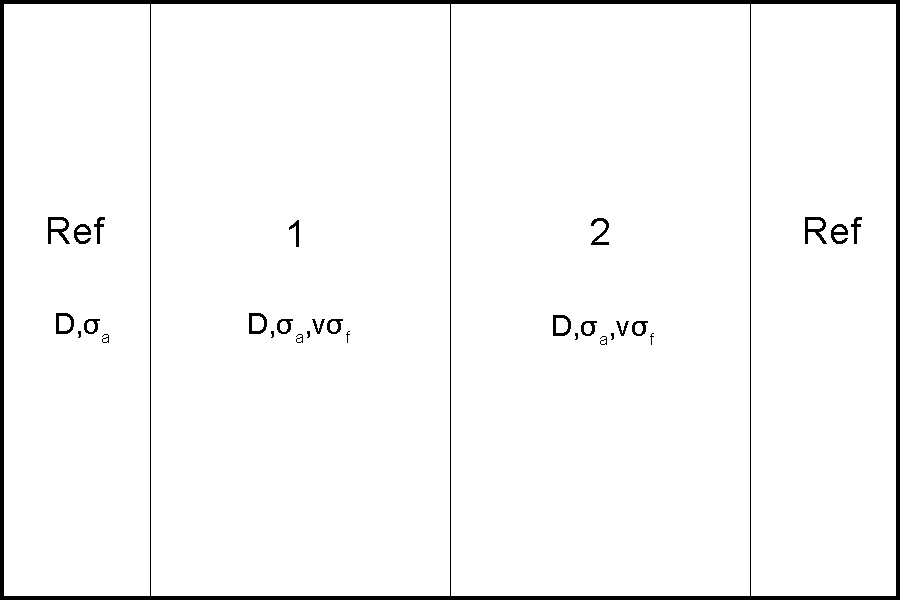
\includegraphics[width=0.5\textwidth]{geom}
   \caption{Problem Geometry}
   \label{geom}
\end{figure}
\subsection{2D Quarter Core problem}
The two-dimensional core is shown in Fig. \ref{coremap}.
\begin{figure}[h!]
\centering
   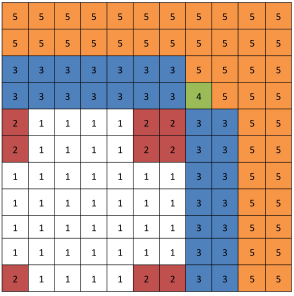
\includegraphics[width=0.5\textwidth]{core}
   \caption{core map}
   \label{coremap}
\end{figure}

\section{Nonlinear Temperature Feedback}

\section{Monte Carlo Sampling}
\subsection{Results}
An example of sampling is introducing 30\% uniform uncertainty in the absorption and fission cross sections.  Using 3000 histories, we arrive at a response surface as shown in Fig. \ref{MCres}.  Each black dot is a sampling point, and the black lines indicate the contours of $k$-eff as a function of changing cross sections.  As expected, the highest $k$ is found when the fission cross section is large and the absorption cross section low.  Interestingly, the fission cross section has a more dominant effect as the absorption cross section increases, and vice versa. 
\begin{figure}[h!]
\centering
   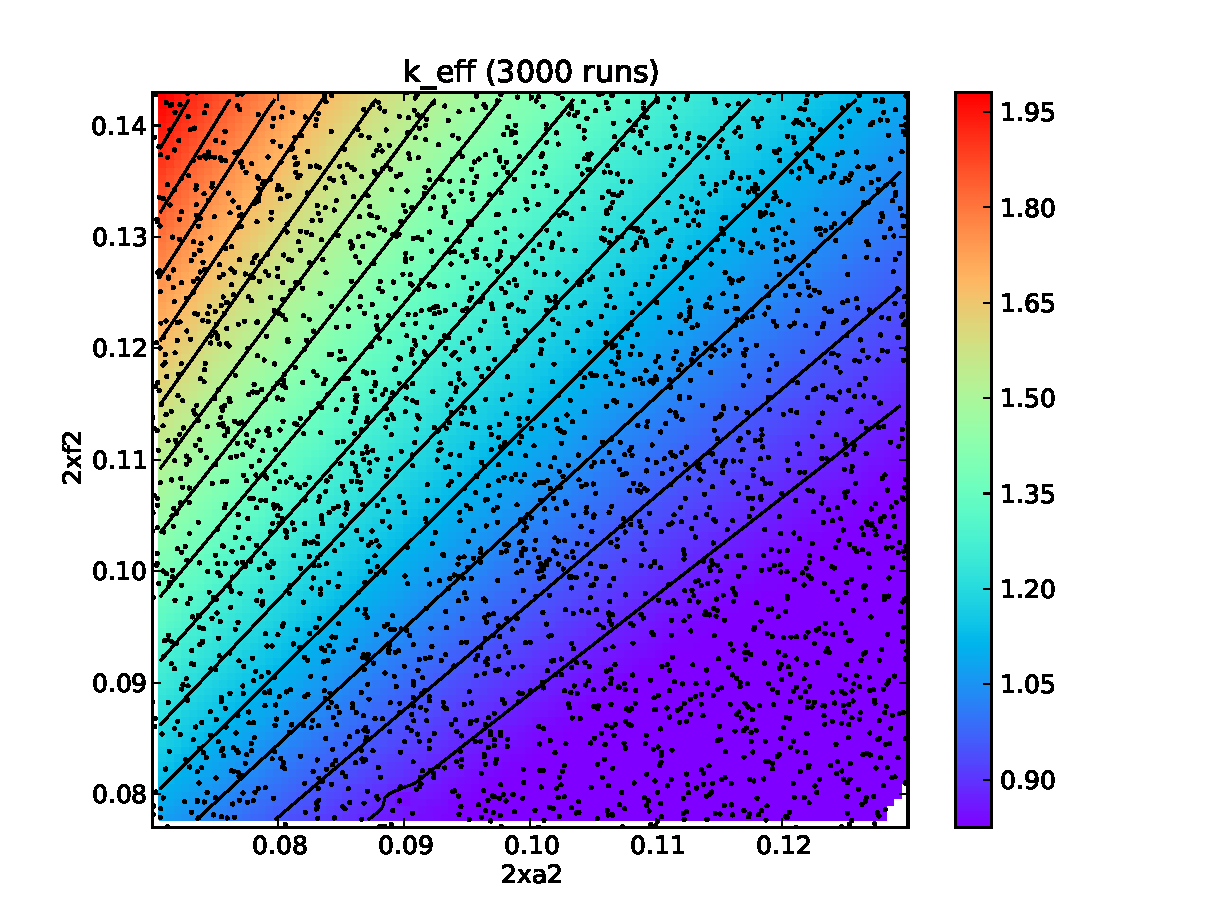
\includegraphics[width=0.7\textwidth]{unc_mc_err30_3000runs}
   \caption{MC Sampling Results}
   \label{MCres}
\end{figure}
\section{Sampling Framework}

\section{Monte Carlo sampling}

\section{Simple Stochastic Collocation sampling}

\section{Mixed Stochastic Collocation sampling}

\section{Sparse Grid Development}

\end{document}

\begin{figure}[h!]
\centering
\includegraphics[width=0.5\linewidth]{1e8sample}
\caption{Distribution of random numbers in 10 bins over 100,000,000 runs.}
\label{1e8sample}
\end{figure}
